
\section{Impulse, Momentum, and Interactions\footnote{
1990-93 Dept. of Physics and Astronomy, Dickinson College. Supported by FIPSE
(U.S. Dept. of Ed.) and NSF. Portions of this material may have been modified
locally and may not have been classroom tested at Dickinson College.
}}

\makelabheader %(Space for student name, etc., defined in master.tex or labmanual_formatting_commands.tex)

\textbf{Objectives }

\begin{itemize}
\item To verify the relationship between impulse and momentum experimentally. 
\item To study the forces between objects that undergo collisions and other types of interactions in a short time period.
\end{itemize}
\textbf{Apparatus} 

\begin{itemize}
\item Collision cart with flag and track 
\item Force probe (force sensor) and bracket
\item Light duty collision spring and hook (for force probe)
\item Motion detector
\item Lab stand
\item CS2000 compact scale
\item Pasco 550 Interface
\item \textit{Capstone} software (\filename{Impulse-Momentum.cap} experiment file)
\end{itemize}
\textbf{The Impulse-Momentum Theorem }

Real collisions, like those between eggs and hands, a tennis ball and a wall, or
a falling ball and a table top are tricky to study because $\Delta t$ 
is so small and
the collision forces are not really constant over the time the colliding objects
are in contact. Thus, we cannot calculate the impulse as $F \,\Delta t$. 
Before we study
more realistic collision processes, let's redo the theory for a variable force.
In a collision, according to Newton's second law, the force exerted on a falling
ball by the table top at any infinitesimally small instant in time is given
by
\begin{equation}
{\vec  F}=\frac{d{\vec  p}}{dt}
\end{equation}

To describe a general collision that takes place between an initial time $t_{i}$
and a final time $t_{f}$ , we must take the integral of both sides of the
equation with respect to time. This gives

\begin{equation}
\int _{t_{i}}^{t_{f}}{\vec  F}dt=\int _{t_{i}}^{t_{f}}\frac{d{\vec  p}}{dt}dt=\left( {{\vec  p}_{f}}-{{\vec  p}_{i}}\right) =\Delta {\vec  p}
\end{equation}

Impulse is a vector quantity defined by the equation
\begin{equation}
{\vec  J}=\int_{t_{i}}^{t_{f}}{\vec  F}\,dt
\end{equation}

By combining equations (2) and (3) we can formulate the impulse-momentum
theorem in which
\begin{equation}
{\vec  J}=\Delta {\vec  p}
\end{equation}

If you are not used to mathematical integrals and how to solve them yet, don't
panic. If you have a fairly smooth graph of how the force $F$ varies as a function
of time, the impulse integral can be calculated as the area under the $F$-$t$ 
curve.

Let's see qualitatively what an impulse curve might look like in a real collision
in which the forces change over time during the collision. In particular, let's
consider the collision of a tennis ball with a wall as shown below.

\vspace{0.3cm}
%{\par\centering \includegraphics{impulse/impulse_fig1.eps} \par}
{\par\centering \includegraphics{impulse/ball_hitting_wall.eps} \par}
\vspace{0.3cm}

\textbf{Activity 1: Predicting Collision Forces That Change }

(a) Suppose a tennis ball is barreling toward a wall and collides with it. If gravity and air friction are neglected, what is the net force exerted on the object just before it starts to collide?
\vspace{10mm}

(b) When will the magnitude of the force on the ball be a maximum? 
\vspace{10mm}

(c) Roughly how long does the collision process take? Half a second? Less? Several
seconds?
\vspace{10mm}

(d) Attempt a rough sketch of the shape of the force the wall exerts on a moving
object during a collision.

%\vspace{0.3cm}
%{\par\centering \includegraphics{impulse/impulse_fig2.eps} \par}
%\vspace{0.3cm}
\begin{lab_axis}*[lab_noticks_1quad,
	width=2in, height=1.4in,
	xlabel=Time,
	ylabel= {Force $F_{\rm wall}$}
]
\end{lab_axis}


\textbf{Verification of the Impulse-Momentum Theorem} 

To verify the impulse-momentum theorem experimentally we must show that for
an actual collision involving a single force on an object the equation
\[
\int_{t_{i}}^{t_{f}}{\vec  F}\,dt=\Delta {\vec  p}\]


holds, where the impulse integral can be calculated by finding the area under
the curve of a graph of $F$ \textit{vs.}~$t$.

%\vspace{0.3cm}
%{\par\centering 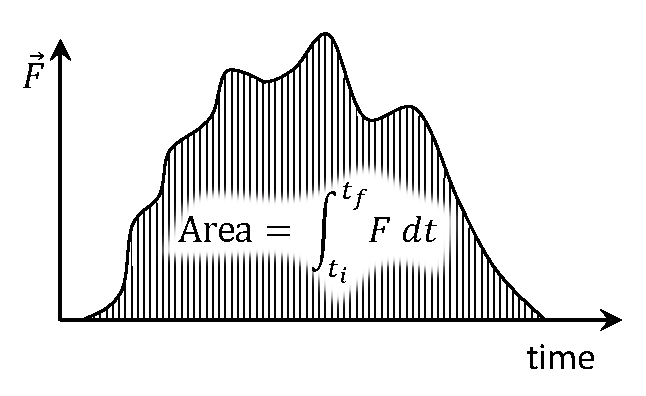
\includegraphics[width=2.5in]{impulse/impulse_fig3_new.eps} \par}
%\vspace{0.3cm}
\begin{lab_axis}*[lab_noticks_1quad,
	width=2.5in, height=1.2in,
	algebraic_labels,
	xlabel=$t$,
	ylabel= $F$,
	xmin=0,xmax=21,
	ymin=0,ymax=10,
]
\addplot +[smooth, tension=0.90, fill= lightgray] coordinates{(0,0) (1,0.5)(3,4) (6,5) (9,8)(11,9)(14,8)(18,1.5)(20,0)};
\addplot +[line width=0.8pt] coordinates{(0,0) (21,0)}; %fixes annoying problem that the fill partially paints over the axis
\node[anchor=south] at (axis cs: 10,0.5)  {Area $\displaystyle =\int_{t_{i}}^{t_{f}}{\vec  F}\,dt$};
\end{lab_axis}

In this experiment you will investigate this theorem by measuring the impulse
and the change in momentum of a cart undergoing a one-dimensional collision.
The experimental setup is shown in the figure below, but with the force probe 
facing the open end of the track so it can be calibrated.  Open the file \filename{Impulse-Momentum.cap} in the \filename{\coursefolder} folder. Calibrate the force probe 
(see \textit{Calibrating Force Sensors} in \textbf{Appendix \ref{capstone}: Capstone}). 
Remove pulley from end of track. Once calibrated, remove the force probe and 
bracket by loosening wing bolts just enough to slide the entire assembly out the 
end of the track. Reverse the assembly and slide the nuts in the slot on the 
other side of the track and tighten wing bolts. Remove hook from force probe and 
replace with light duty collision spring. The setup should now look like the figure 
below.

The end of the track with the motion detector should be raised (using lab stand) 
about 1.5 cm so that, when released, the cart will collide with the force probe. 
The force probe will measure the force as a function of time during the collision. 
The motion detector is used to measure the velocity of the glider before and after the 
collision. You will use the Impulse-Momentum application to make these measurements.

\vspace{0.3cm}
{\par\centering \resizebox*{0.9\textwidth}{!}{\includegraphics{impulse/impulse_fig4.eps}} \par}
\vspace{0.3cm}

\textbf{Activity 2: Verification of the Impulse-Momentum Theorem} 

(a) Measure the mass of the cart, $m$, using the compact scale, and record it here:
\vspace{10mm}

(b) Construct a data table in the space below with the column headings Trial
\#, Area, \( v_{i} \), and \( v_{f} \). Make enough room to record 6-8 trials.

\newpage

%(c) Position the force probe part way up the track (to be closer to the motion sensor).

(c) Set the cart on the track about mid-way between the motion sensor and the force probe. Start recording data and release the cart. Stop recording data after the cart collides with the force probe and bounces back. The computer will then display graphs of velocity and force versus time.

(d) Determine the area under the force \textit{vs.}~time graph and record the value in
your data table. See \textbf{Appendix \ref{capstone}: Capstone} for instructions on how to determine the area under a curve.

(e) Use the \textbf{Delta Tool} function to find the velocity just before the collision and the
velocity just after the collision from the velocity versus time graph. Use the 
PEAK values (positive and negative), even if they do not coincide with where 
the force curve begins and ends. Be sure and record emph{velocity} values 
(the second number in the Delta Tool reading), not time values. 
Record these values in your data table.

(f) Repeat parts (c) through (e) 5-7 times, setting the cart at the same place on the track for each trial. \textbf{Note:} For these trials, the area function and the Delta Tool must be turned off and on for each trial. Print the graphs for one of your trials and include it with this report.

(g) Construct another data table below with the column headings
Trial \#, $J$, \( \Delta  p\), Diff., and Percent diff. For each trial, record
the impulse, $J$, and calculate and record the change in momentum, \( \Delta  p\), in kg\,m/s. Also, determine the difference between $J$ and $\Delta p$  for 
each trial, and the percent difference. Alternatively, this table can be constructed in \textit{Excel}, and the calculations done there. Include table with this unit.
%Also, show a sample calculation of $I$ and \( \Delta  p\) for one of your trials.
\vspace{60mm}

(h) What do you expect for the values in the last column of your table (Percent diff)? Make a histogram of your results in that column and calculate the average and standard deviation. For information on making histograms, see \textbf{Appendix \ref{excel}}. For information on calculating the average and standard deviation, see \textbf{Appendix \ref{treatment}} (can also be done in \textit{Excel}). Record the average and standard 
deviation here. Attach the histogram to this unit. Is your data consistent with your expectation?
\vspace{15mm}

(i) Do your results verify the impulse-momentum theorem? Explain quantitatively.
\vspace{15mm}

(j) What does the histogram of your data tell you?
\vspace{15mm}

(k) Is there any indication of a systematic uncertainty? What are the possible
sources of error?

